\section{Isothermal Annealing Studies}
\label{sec:annealing}

\begin{figure}
	\captionsetup[subfigure]{aboveskip=-1pt,belowskip=-1pt}
	\centering
	\begin{subfigure}[b]{0.49\textwidth}
		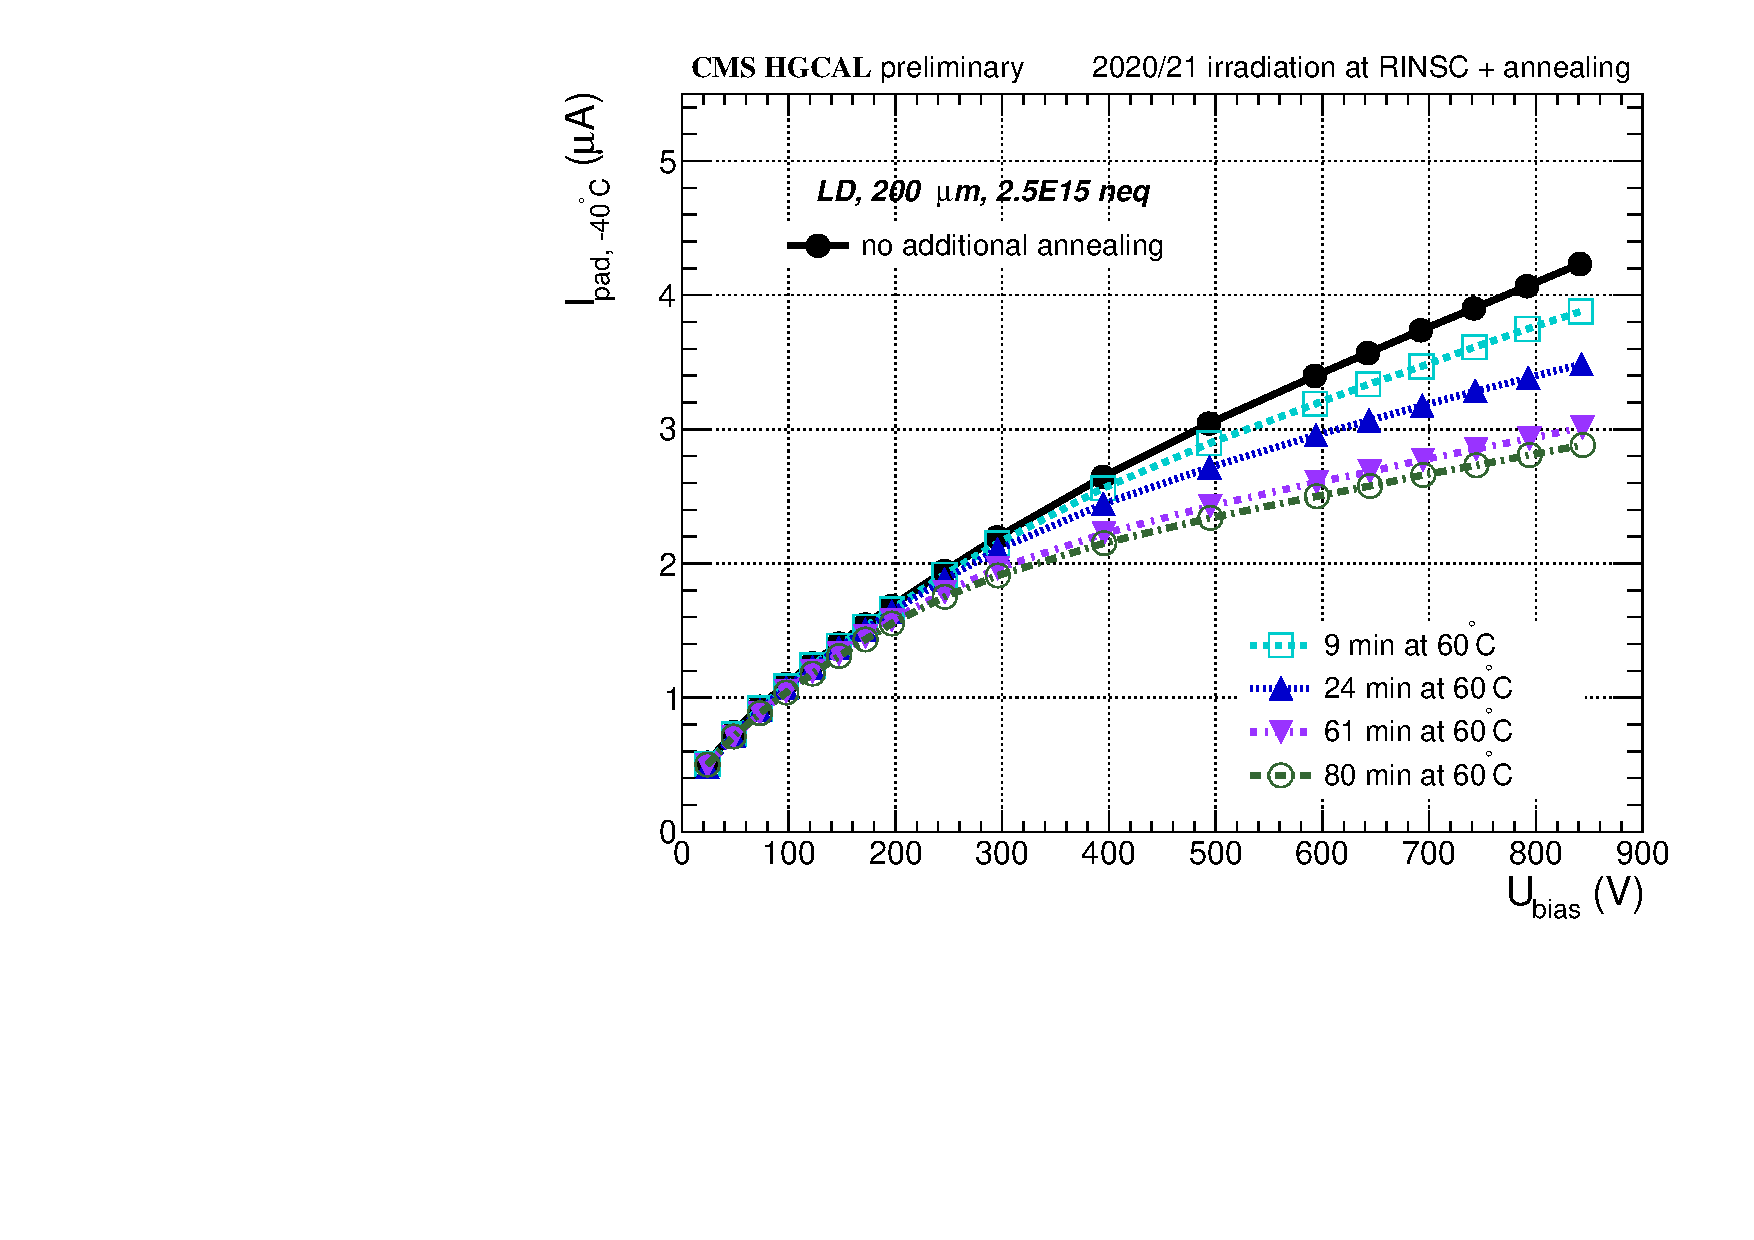
\includegraphics[width=0.999\textwidth]{plots/annealing_iv/annealing_IV_ch24.pdf}
		\subcaption{
		}
		\label{plot:annealing_IV}
	\end{subfigure}
	\hfill
	\begin{subfigure}[b]{0.49\textwidth}
		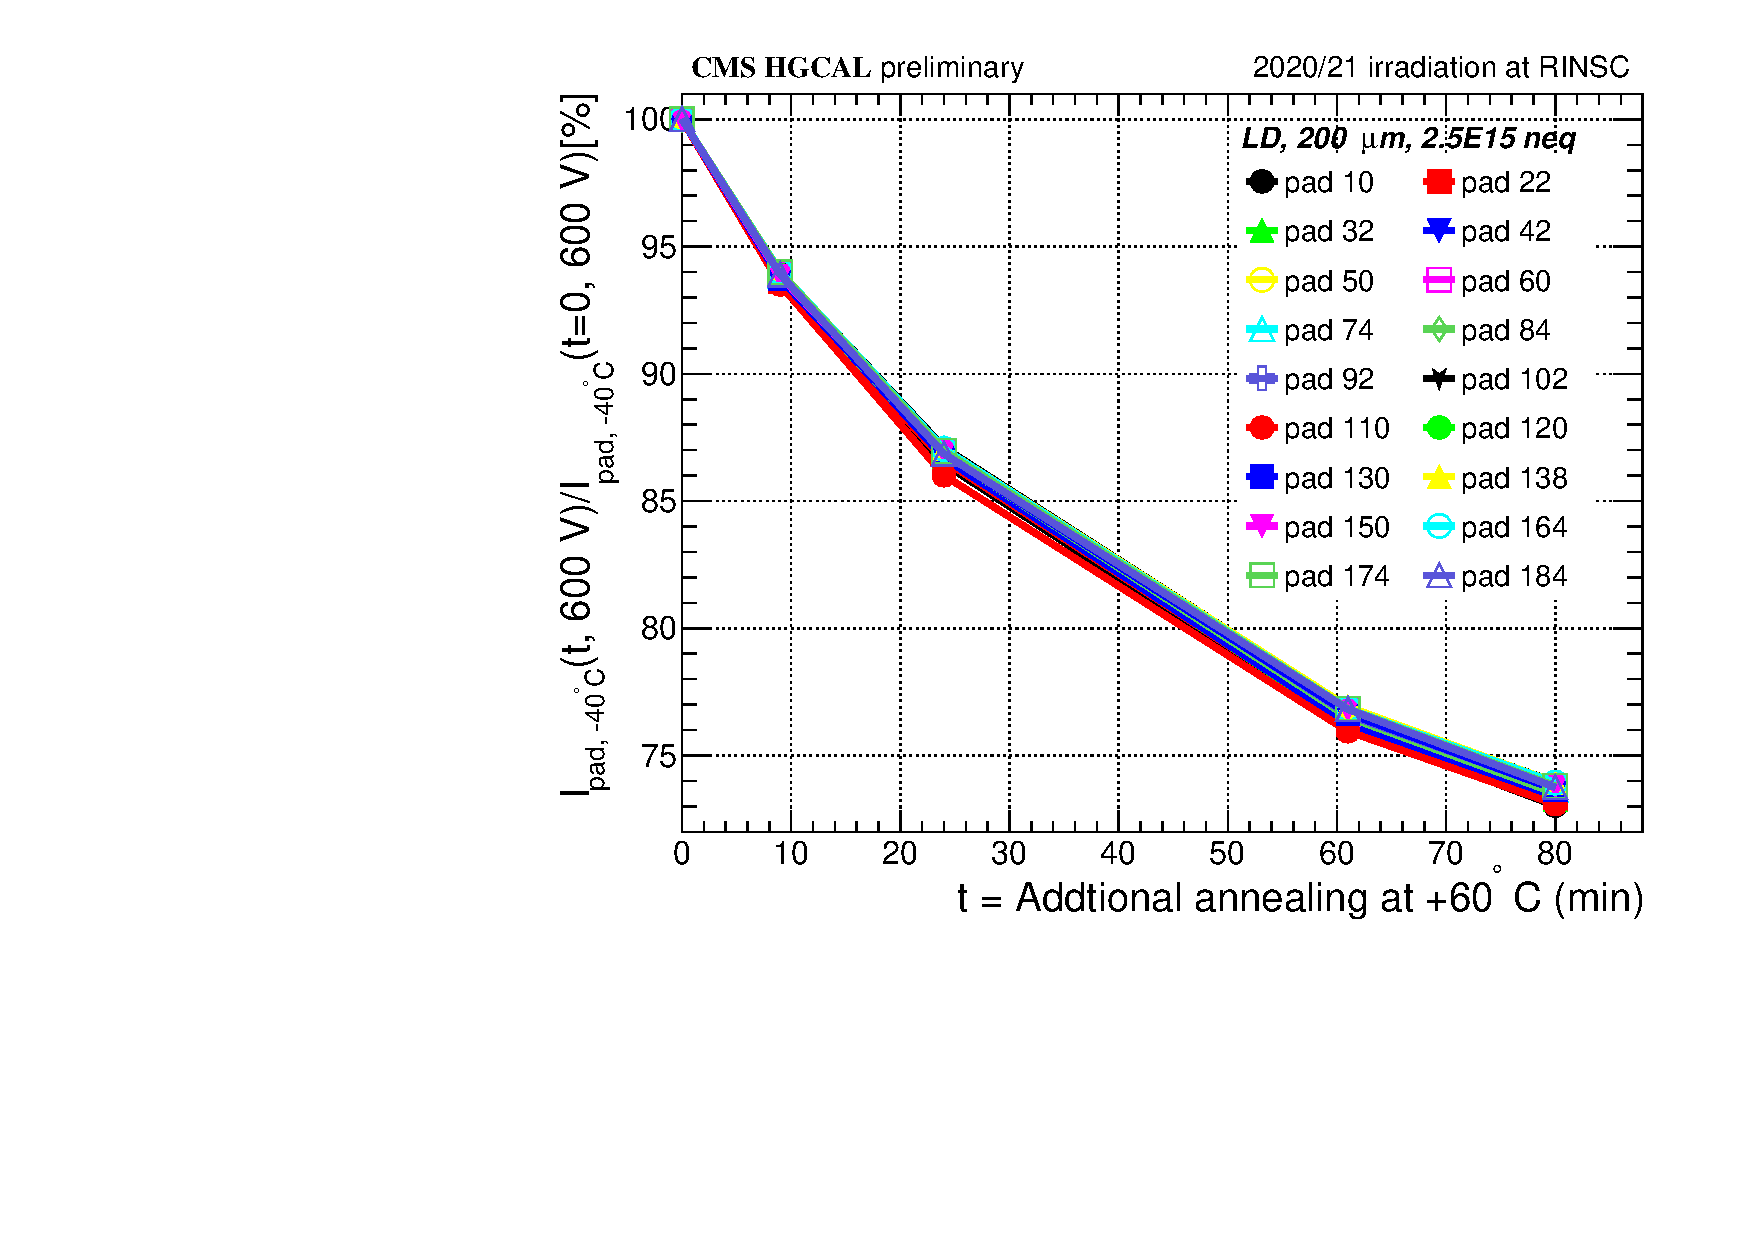
\includegraphics[width=0.999\textwidth]{plots/annealing_iv/annealing_current.pdf}
		\subcaption{
		}
		\label{plot:annealing_current}
	\end{subfigure}
	\caption{
		(a) Representative per-pad IV-curves for different annealing scenarios for a \SI{200}{\micro\metre} low-density prototype sensor irradiated to 2.5$~$E15 1-MeV-neutron equivalents/cm$^{2}$.
        (b) Decrease of the per-pad leakage current (interpolated to $U_\text{bias}=\SI{600}{\volt}$) as a function of the additional annealing time at \SI{60}{\celsius}.
	}
\end{figure}